\chapter{DESAIN DAN PERANCANGAN}
    Pada bab ini dibahas mengenai analisis dan perancangan sistem.
    
    \section{Deskripsi Umum Sistem}
    	\indent Sistem yang akan dibangun pada tugas akhir ini adalah sebuah sistem yang dapat melakukan automasi uji beban terhadap suatu web. Uji beban pada sistem akan berjalan secara \textit{headless} menggunakan sebuah \textit{tester} yaitu \textit{Headless Chrome}. \textit{Headless Chrome} akan mendapatkan data uji beban ketika mengakses web yang diuji, sedangkan yang digunakan untuk mengambil data uji beban adalah sebuah pustaka \textit{Node} yaitu \textit{Puppeteer}. Sistem juga akan menggunakan \textit{Docker} sebagai infrastruktur, sehingga \textit{Docker} dapat digunakan sebagai \textit{load generator} untuk melakukan uji beban yang bisa disebut kontainer.
    	
    	\indent Kontainer yang akan dipasang pada sistem membutuhkan sebuah alat orkestrasi untuk memanajemen kontainer secara otomatis, alat orkestrasi yang digunakan adalah \textit{Docker Swarm}. \textit{Docker Swarm} akan melibatkan 3 \textit{node host} yang akan dibagi menjadi 1 \textit{node host} sebagai \textit{swarm manager} dan 2 \textit{node host} sebagai \textit{worker}. \textit{Docker Swarm} akan bertanggung jawab dalam mendistribusikan kontainer ke masing-masing \textit{swarm node} yang tergabung pada lingkungan \textit{swarm} atau bisa disebut sebagai \textit{load balancer}.
    	
    	\indent Proses uji beban akan diproses ketika pengguna melakukan \textit{request} skenario uji beban pada \textit{web service} yang disediakan sistem. Kemudian \textit{controller} pada \textit{web service} akan mengirimkan skenario uji pada kontainer terpilih untuk melakukan pengujian. Setiap kontainer akan terinstall \textit{Headless Chrome} dan \textit{Puppeteer}. \textit{Headless Chrome} akan mendapatkan data uji beban dan automasi pengambilan data uji beban dilakukan oleh \textit{Puppeteer}. \textit{Puppeteer} akan melakukan ekstraksi data uji beban menjadi satuan \textit{millisecond(ms)}. 
    	
    	\indent Sistem akan menyediakan basis data untuk menyimpan data yang diperlukan sistem. Basis data akan dipasang diluar lingkungan swarm dan lingkungan \textit{web service}. Sistem juga menyediakan antarmuka pengguna berupa web yang akan digunakan untuk melihat laporan hasil uji beban. Sedangkan untuk mengatasi \textit{multiuser}, sistem akan menggunakan \textit{task scheduler(crontab)} dan \textit{queue}(antrian).
    
    \section{Kasus Penggunaan}
	    \begin{figure}[H]
	    	\centering
	    	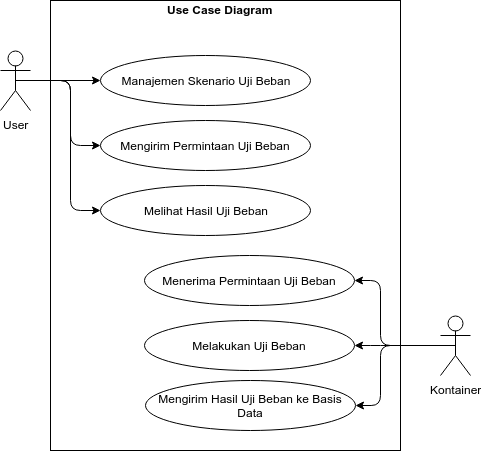
\includegraphics[width=9cm,height=9cm]{Images/C-3/usecasediagram.png}
	    	\caption{Diagram kasus penggunaan}
	    	\label{usecased}
	    \end{figure}
    	Terdapat dua aktor dalam sistem yang akan dibuat yaitu \textit{User} dan Kontainer. \textit{User} merupakan aktor(pengguna) yang bisa melakukan manajemen pada skenario yang ingin diuji dan melihat hasilnya, sedangkan Kontainer merupakan aktor yang akan digunakan sebagai \textit{load generator} untuk melakukan uji beban. Diagram kasus penggunaan digambarkan pada Gambar \ref{usecased} dan dijelaskan masing-masing pada Table \ref{tabelusecase}.
    	
    	\begin{longtable}{|p{0.20\textwidth}|p{0.30\textwidth}|p{0.35\textwidth}|}
    		\caption{Daftar kode kasus penggunaan} \label{tabelusecase} \\
    		\hline
    		\textbf{Kode Kasus Penggunaan} & \textbf{Nama Kasus Penggunaan} & \textbf{Keterangan} \\ \hline
    		\endhead
    		\endfoot
    		\endlastfoot
    		UC-0001 & Manajemen Skenario Uji Beban & \textit{User} dapat menambah, melihat dan menghapus skenario uji beban \\ \hline
    		UC-0002 & Mengirim Permintaan Uji Beban & \textit{User} dapat mengirimkan permintaan uji beban ke sistem melalui \textit{web service} yang disediakan \\ \hline
    		UC-0003 & Melihat Hasil Uji Beban & Ketika proses uji beban selesai, \textit{user} dapat melihat hasilnya di antarmuka pengguna \textit{web service} yang disediakan \\ \hline
    		UC-0004 & Menerima Permintaan Uji Beban & Proses dimana kontainer akan menerima permintaan uji beban dari \textit{User} \\ \hline
    		UC-0005 & Melakukan Uji Beban & Proses dimana kontainer akan melakukan uji beban sesuai skenario yang dikirim \\ \hline
    		UC-0006 & Mengirim Hasil Uji Beban ke Basis Data & Ketika kontainer telah selesai melakukan pengujian, data yang didapatkan akan dikirim ke basis data \textit{MySQL} \\ \hline
    	\end{longtable}
    
    \section{Arsitektur Sistem}
	    \begin{figure}[H]
	    	\centering
	    	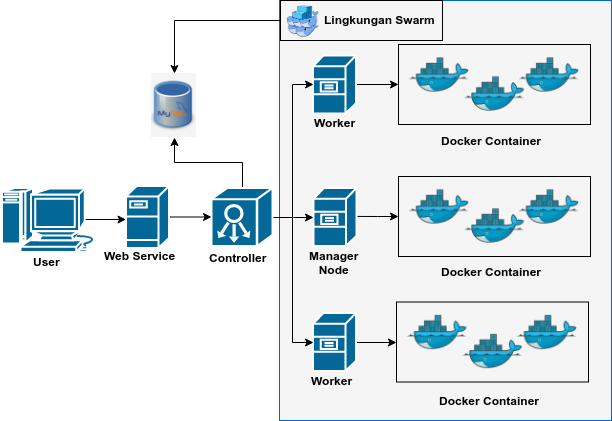
\includegraphics[width=10cm,height=6cm]{Images/C-3/arsitektursistem.png}
	    	\caption{Desain arsitektur sistem}
	    	\label{arsitekturumum}
	    \end{figure}
    	
    	\indent Pada sub-bab ini, akan dibahas mengenai tahap analisis arsitektur, analisis teknologi dan desain sistem yang akan dibangun. Arsitektur sistem secara umum ditunjukkan pada Gambar \ref{arsitekturumum}.

    	\subsection{Desain Umum Sistem}
    		Berdasarkan yang dijelaskan pada deskripsi umum sistem, dapat diperoleh beberapa kebutuhan sistem antara lain:
    		\begin{enumerate}
    			\item \textit{Load generator} untuk melakukan uji beban.
    			\item \textit{Tester} yang bisa mengambil data uji beban.
    			\item \textit{Web service} sebagai antarmuka pengguna.
    			\item Basis data untuk menyimpan data sistem.
    			\item \textit{Task queue} untuk menangani kasus \textit{request} lebih dari satu user.
    		\end{enumerate}
    	
    		Untuk memenuhi kebutuhan sistem yang dijelaskan sebelumnya, penulis membagi menjadi beberapa komponen sistem yang akan digunakan pada tugas akhir ini.
    		
    		\begin{enumerate}
    			\item \textit{Load generator} \\
    				Berfungsi sebagai pengganti user yang akan melakukan akses web melalui \textit{browser}.
    			\item Pengambil data uji beban \\
    				Berfungsi untuk mengambil data uji beban ketika \textit{load generator} mengakses web dari \textit{browser}.
    			\item \textit{Service Controller} \\
    				Berfungsi sebagai pengatur sistem uji beban yang terdiri :
    				\begin{itemize}
    					\item \textit{Web Service} \\
    						Berfungsi sebagai tampilan antarmuka pengguna untuk menggunakan sistem.
    					\item Basis Data \\
    						Berfungsi untuk menyimpan data yang digunakan untuk menyimpan segala data yang dibutuhkan oleh sistem.
    					\item \textit{Task Queue} \\
    						Berfungsi untuk membuat \textit{task scheduler} dan antrian untuk menangani kasus \textit{request} lebih dari satu user.
    				\end{itemize}
    		\end{enumerate}
    	
    	\subsection{Perancangan \textit{Load Generator}}
	    	\begin{figure}[h]
	    		\centering
	    		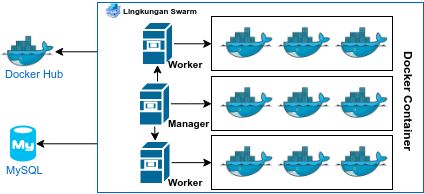
\includegraphics[width=11cm,height=6cm]{Images/C-3/dockerdesain.png}
	    		\caption{Desain perancangan \textit{load generator}}
	    		\label{dockerdesain}
	    	\end{figure}
    		Komponen \textit{load generator} akan difungsikan sebagai pengganti pengguna yang mengakses ke suatu web melalui \textit{browser}. Komponen yang akan digunakan sebagai \textit{load generator} adalah \textit{Docker} atau bisa disebut kontainer. Ketika melakukan pemasangan kontainer sebuah \textit{Docker Image}, untuk memenuhi hal tersebut, pada tugas akhir ini penulis akan membuat sebuah \textit{Docker Image} yang akan diunggah ke \textit{Docker Hub}. Sehingga ketika akan memasang kontainer pada \textit{node host} yang baru, node host tersebut hanya perlu mengunduh \textit{Docker Image} yang telah diunggah sebelumnya. Seluruh kontainer akan dibangun di dalam lingkungan \textit{swarm} untuk memudahkan dalam mengatur atau memanajemen kontainer ke semua \textit{node host} yang tergabung di dalam lingkungan \textit{swarm}, sedangkan untuk memudahkan akses ke setiap kontainer, maka data dari kontainer akan disimpan di dalam basis data \textit{MySQL}. \textit{Load generator} akan terdiri dari 3 \textit{node host}, 1 sebagai \textit{manager node} dan 2 lainnya sebagai \textit{worker}, sedangkan basis data akan berada di luar lingkungan \textit{swarm}. Desain perancangan komponen ini digambarkan pada Gambar \ref{dockerdesain}.
    		 
    	
    	\subsection{Perancangan Pengambil Data Uji Beban}
    		Komponen ini akan membutuhkan suatu alat yang bisa mendapatkan data uji beban terlebih dahulu. Pada tugas akhir ini, akan menggunakan \textit{Headless Chrome} untuk mendapatkan data uji beban ketika mengakses web. Setelah mendapatkan data uji beban, diperlukan juga suatu alat yang bisa digunakan untuk mengambil data uji beban pada \textit{Headless Chrome}, alat tersebut adalah \textit{Puppeteer}. \textit{Puppeteer} akan melakukan pengambilan secara otomatis ketika ada perintah yang masuk dan menyimpan data uji beban pada basis data \textit{MySQL}. Alat-alat yang digunakan pada komponen ini akan dipasang pada masing-masing kontainer di setiap \textit{node host}. Desain perancangan komponen ini digambarkan pada Gambar \ref{puppdesain}.
    		\begin{figure}[H]
    			\centering
    			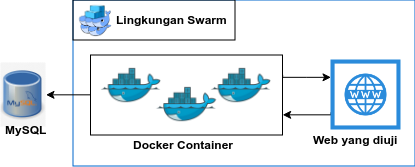
\includegraphics[width=10cm,height=4.5cm]{Images/C-3/puppdesain.png}
    			\caption{Desain pengambil data uji beban}
    			\label{puppdesain}
    		\end{figure}
    	
    	\subsection{Perancangan \textit{Service Controller}}
    		Komponen ini akan digunakan untuk mengatur segala proses uji beban pada sistem. Pada komponen ini akan terdapat 3 buah sub-komponen yaitu \textit{web service}, basis data dan \textit{task queue} atau antrian.
    	
	    	\subsubsection{Desain \textit{Web Service}}
	    		\textit{Web service} akan berfungsi sebagai antarmuka pengguna dan sebagai penghubung antara pengguna dengan kontainer. Antarmuka pengguna berfungsi memudahkan pengguna untuk membuat skenario yang akan dikirimkan ke \textit{load generator} dan kemudian \textit{load generator} akan melakukan uji beban sesuai dengan skenario yang dikirim melalui \textit{web service}. Sedangkan untuk mengatur segala aktivitasnya dibutuhkan sebuah \textit{controller} dan rute yang akan dipasang pada \textit{web service}. Desain antarmuka pengguna ditunjukkan pada Gambar \ref{mockupweb}.
	    		\begin{figure}[H]
	    			\centering
	    			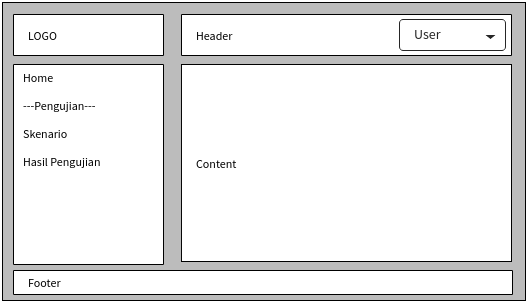
\includegraphics[width=10cm,height=6cm]{Images/C-3/mockupweb.png}
	    			\caption{Desain antarmuka pengguna}
	    			\label{mockupweb}
	    		\end{figure}
	    	
		    	Selain itu, akan dirancang juga fitur-fitur pada \textit{web service} yang akan digunakan pengguna antara lain:
		    	\begin{enumerate}
		    		\item Menambah dan menghapus skenario.
		    		\item Menentukan jumlah \textit{load generator} pengujian.
		    		\item Melihat performa hasil pengujian.
		    		\item Melihat tangkapan layar tampilan web yang diuji.
		    		\item Melihat \textit{console error}.
		    		\item Melihat status antrian proses uji. \\
		    	\end{enumerate}
	    		
	   		\subsubsection{Desain Basis Data}
	   			Komponen basis data diperlukan untuk menyimpan data-data yang berkaitan dengan sistem. data yang disimpan adalah data \textit{node host swarm}, data kontainer, data pengguna, data skenario pengujian, data antrian \textit{request}, data hasil pengujian, data \textit{error console}, data rata-rata hasil pengujian. Dari data-data tersebut maka dibutuhkan suatu tabel diantaranya yaitu:
	   			\begin{itemize}
	   				\item Tabel \textit{swarms} \\
	   					Menyimpan data \textit{nohe host} yang tergabung di dalam lingkungan \textit{swarm}.
	   				\item Tabel \textit{containers} \\
	   					Menyimpan data \textit{Docker Container} yang telah dipersiapkan.
	   				\item Tabel \textit{users} \\
	   					Menyimpan data pengguna.
	   				\item Tabel \textit{scenarios} \\
	   					Menyimpan data skenario pengujian.
	   				\item Tabel \textit{queues} \\
		   				Menyimpan data antrian \textit{request} pengujian dari pengguna.
	   				\item Tabel \textit{results} \\
	   					Menyimpan data hasil pengujian yang dilakukan setiap kontainer.
	   				\item Tabel \textit{errors} \\
	   					Menyimpan data \textit{console error} yang ada di \textit{browser}.
	   				\item Tabel \textit{summary results} \\
	   					Menyimpan data rata-rata hasil pengujian setiap skenario.
	   			\end{itemize}
	    		
	    	\subsubsection{Desain Penggunaan \textit{Task Queue}}
	    		Pada \textit{service controller} akan ada banyak \textit{request} dari pengguna, setiap \textit{request} tentu saja akan terdapat proses yang akan berjalan dalam jangka waktu yang cukup lama. Jika proses tersebut berada di dalam fungsi yang dipanggil melalui protokol \textit{HTTP}, maka akan memberikan umpan balik setelah semua proses yang ada dibaliknya selesai. Hal ini akan membuat pengguna yang melakukan \textit{request} perlu menunggu dan tidak efisien. Untuk mengatasi hal ini, akan dirancang sebuah komponen antrian atau bisa disebut \textit{task queue}. \textit{Task queue} akan membuat antrian untuk setiap \textit{request} dibelakang layar. Antrian \textit{request} tersebut akan disimpan pada basis data \textit{MySQL}.